\section{Mathematical relations}

\subsection{Relation of Daily Radiation and PAR}

En HortSys, considera  solo el $50\%$ de las frecuencias recibidas son utilizadas para la producción de carbohidratos.
        
        \begin{gather}
            \mathcal{G}_{par} = \frac{u_{R}}{2}
            \hspace{1em} \Rightarrow \hspace{1em}
            y_{par}(t) = \mathcal{G}_{par} (u_{R})
        \end{gather}


\subsection{Relation LAI and PTI}

En \cite{Martinez-Ruiz2019} LAI es considerado una variable  dependiente de la variable de estado \emph{Photothermal Time} ($x_{pt}$), siguiente la siguiente relación:
\begin{gather}
    \mathcal{G}_{la}(z) =  \frac{z}{c_2 + z}c_1 d    
    \hspace{1em} \Rightarrow \hspace{1em}
    y_{la} = \mathcal{G}_{la}(x_{pt})
\end{gather}

Donde $d$ es densidad de plantas por metro cuadrado.

Cabe mencionar la correspondencia de comportamiento asintótico de la relación anterior con la experiencia observada (Figure \ref{fig:Gla}). 
\begin{enumerate}
    \item  Cuando $x_{pt} << c_2 $ esperamos un comportamiento lineal entre $  y_{la} \approx (c_1 d/c_2) x_{pt} $.
    \item Cuando $x_{pt} \to \infty $ entonces $y_{la} \to c_1 d$. Es decir, si recordamos que $x_{pt}$ representa el cantidad de energía solar acumulada, podemos notar que este modelo predice una relentización y luego un estancamiento del área total de las hojas. Esto se puede interpretar como un balance, entre la maximización en la recepción de radiación y el mantenimiento de estos órganos.
    
\end{enumerate}

\begin{figure}
    \centering
    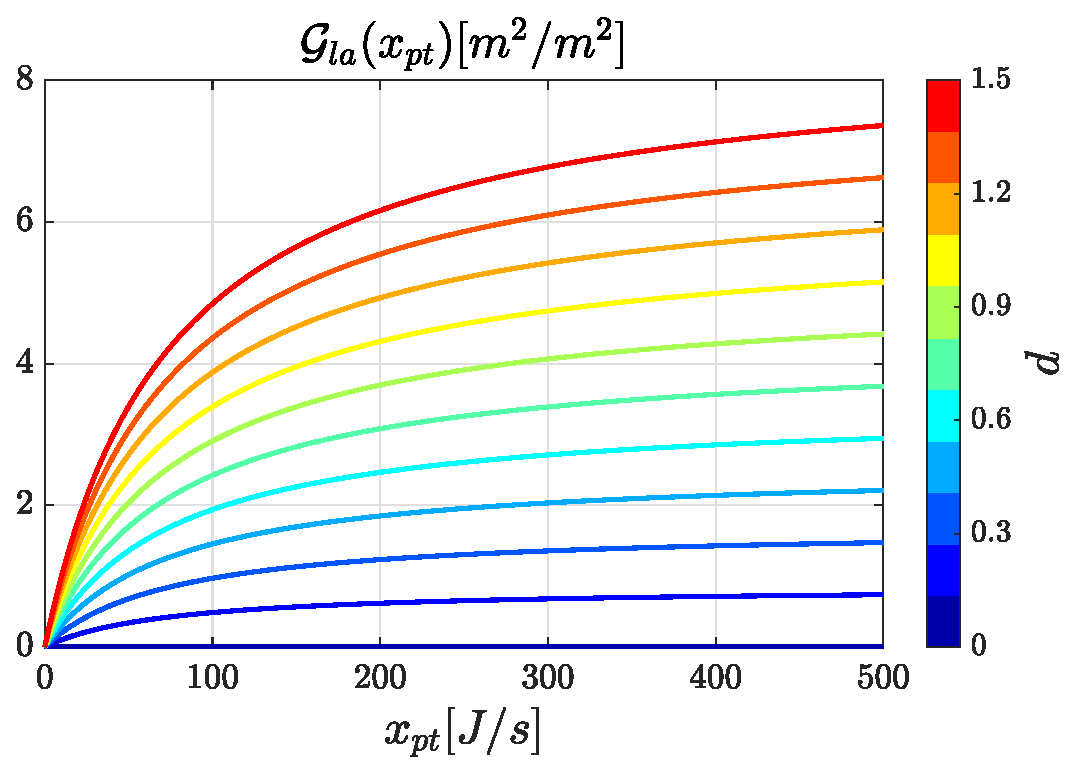
\includegraphics[scale=0.5]{img/gla.eps}
    \caption{$\mathcal{G}_{la}$ para distintos valores de $d$. Se puede ver que el valor de \emph{Leaf Area Index} se satura según aumenta el valor de $x_{pt}$. En concreto toma el valor de saturación  $y_{la} = c_1d$. Es decir el area de hoja máxima es proporcional a la densidad de superfice de plantas.}
    \label{fig:Gla}
\end{figure}
    
\subsection{Relation LAI and FPAR}

Se considera que depende del LAI de la siguiente manera:
\begin{gather}
    \mathcal{G}_{fpar}(z) = 1 - e^{-k z}
    \hspace{1em} \Rightarrow \hspace{1em}
    y_{fpar} = \mathcal{G}_{fpar}(y_{la})
\end{gather}


\subsection{Relation: FPAR \& PTT}

Con el fin de simplificar las expresiones podemos definir la siguiente función ($\mathcal{F}: \mathbb{R}^2 \rightarrow \mathbb{R}$). Esta es la función que tomando el valor de radiación diaria y Photothermal time devuelve un ratio de crecimiento común para las variables $x_{pt}$ y $x_{dmp}$
\begin{gather}
    \mathcal{F}_{fpar}(x_{pt}) =   \mathcal{G}_{fpar}[ \mathcal{G}_{la}(x_{pt})]
\end{gather}
Desarrollando la expresión
\begin{gather}
    \mathcal{F}_{fpar}(x_{pt}) =   
        1- \exp \Big(-\frac{c_1x_{pt}}{c_2+x_{pt}} kd\Big)
        \hspace{1em} 
        \Rightarrow 
        \hspace{1em} 
        y_{fpar} = \mathcal{F}_{fpar}(x_{pt})
\end{gather}

Comportamiento asintótico (Figure \ref{fig:Fpar})
\begin{enumerate}
    \item Cuando $x_{pt} \to \infty$ el valor de $y_{fpar} \to 1 - \exp(-kc_1 d/c_2)$. Es decir, la fracción interceptada para cualquier condición initial del sistema siempre se saturará en este valor.
\end{enumerate}
\begin{figure}
    \centering
    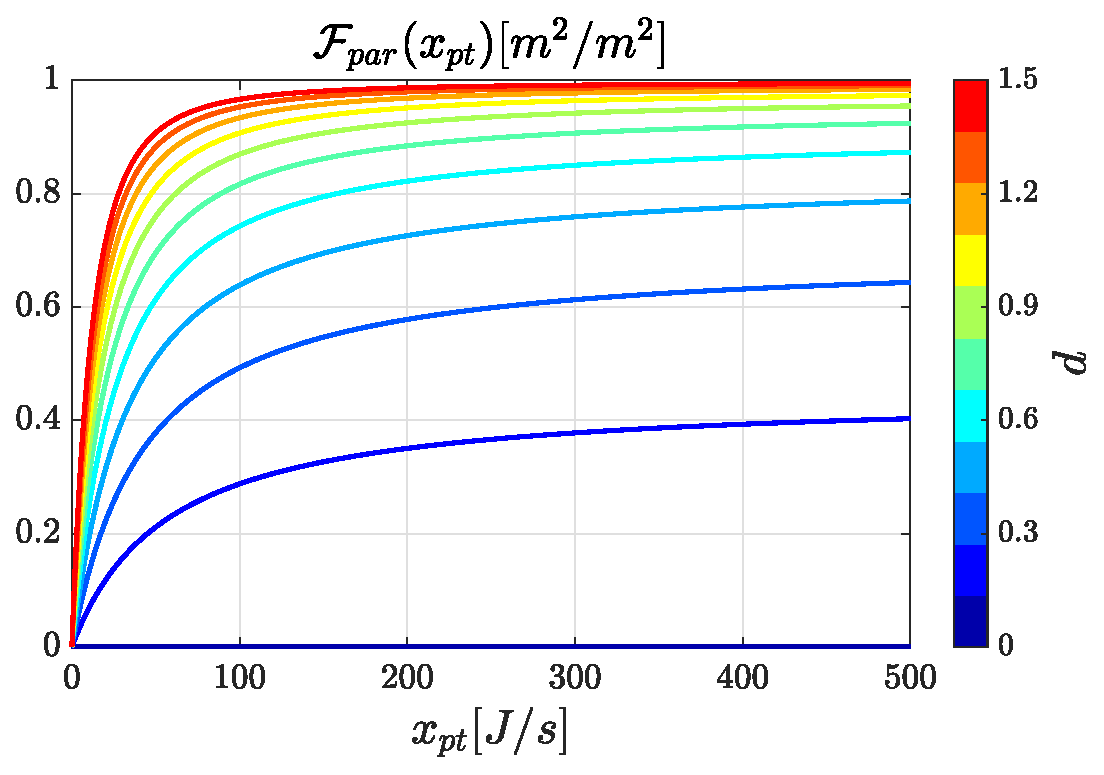
\includegraphics[scale=0.5]{img/F_x_pt.eps}
    \caption{Fraction de radación captada debido conrespecto al valor de $x_{pt}$. }
    \label{fig:Fpar}
\end{figure}  



\section{Metabolical effects by climate variables}



\subsection{Inhibición de crecimiento por Temperatura} ($\mathcal{G}_T^d:\mathbb{R} \rightarrow \mathbb{R}$): Tomado del \cite{Martinez-Ruiz2019} 
\begin{gather}
    \mathcal{G}_T^d(z) = \begin{cases}
        0 & z<T_{min} \\
        (z-T_{min})/(T_{ob} - T_{min}) & T_{min} < z < T_{ob} \\
        1 & T_{ob} \leq z <\leq T_{ou} \\
        (T_{max}-z)/(T_{max}- T_{ou}) & T_{ou}< z < T_{max} \\
        0 & z>T_{max}
    \end{cases}
\end{gather}
{Función de inhibición de Temperatura Suavizada} ($\mathcal{G}_{T}:\mathbb{R} \rightarrow \mathbb{R}$): Consideraremos una función de inibición de crecimiento, de manera que la recepción de radiación solo es posible dentro de uno rango concreto de temperatura. De manera que podemos escribir esta función como:
\begin{gather}\label{GTT01}
    \mathcal{G}_{T}(z) = 
    1-h_{\eta}(z-T_{max})-h_{\eta}(T_{min}-z) 
\end{gather}
Donde $h_{\eta}$ es un aproximación suave de la función escalón
\begin{gather}
    h_{\eta}(z) = [1+\tanh(\eta z)]/2 
\end{gather}
De manera que podemos reescribir \eqref{GTT01} como:
\begin{gather}
    \mathcal{G}_{T}(z) = -\frac{1}{2} \tanh[\eta_{max}(z-T_{max})] - \frac{1}{2}\tanh[\eta_{min} (T_{min}-z)]
\end{gather} 
De manera que esta función tiene el valor de uno cuando la temperatura se encuentra en el intervalo $[T_{min},T_{max}]$ y cero fuera de él. 
\begin{figure}[ht!]
    \centering
    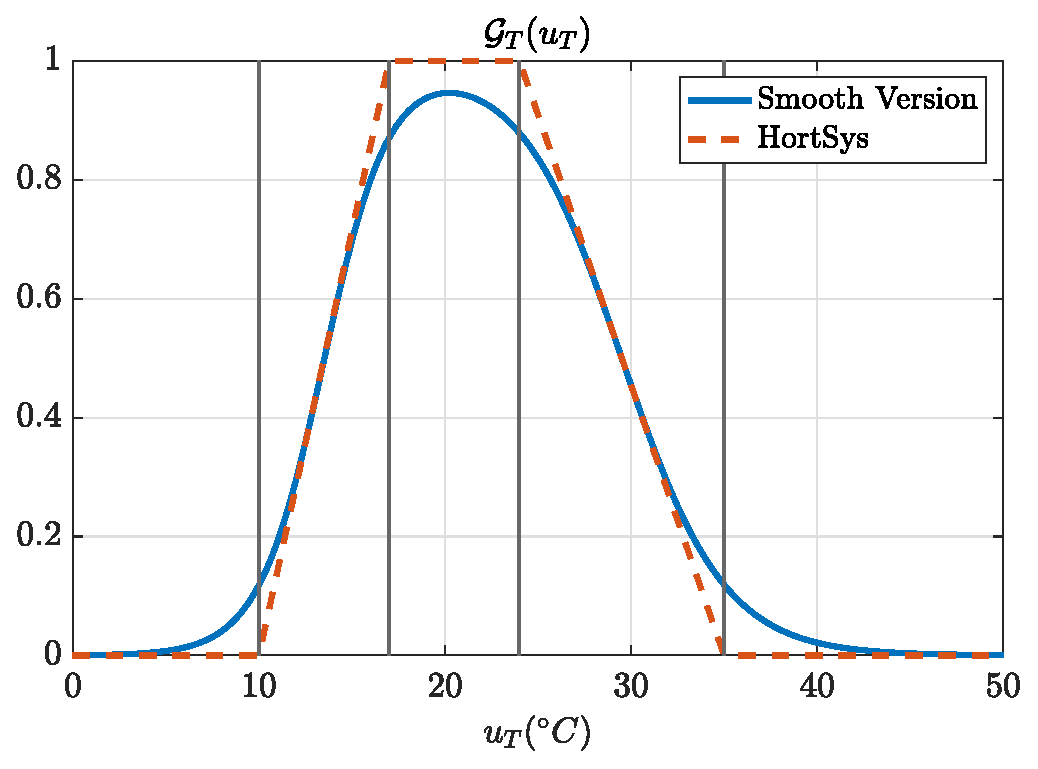
\includegraphics[scale=0.5]{img/uT_sm.eps}
    \caption{Función de inibición de crecimiento por temperatura}
    % T00
\end{figure}